%&tex

\documentclass[14pt]{ffslides}

\ffpage{40}{1.7777}

\usepackage{helvet}
\usepackage[english]{babel}
\usepackage[utf8]{inputenc}
\usepackage[T1]{fontenc}
\usepackage{wrapfig}
\usepackage{csquotes}
\usepackage{mathtools}
\usepackage{amsfonts}
\usepackage{amsthm}
\usepackage{amssymb}
\usepackage{thmtools,thm-restate}
\usepackage{multicol}
\usepackage{hyperref}
\usepackage{graphicx}
\usepackage{pifont}
\usepackage[singlelinecheck=false]{caption}
\usepackage{algorithm}
\usepackage[noend]{algpseudocode}
\usepackage{subcaption}
\usepackage{booktabs}
\usepackage{textcomp}
\usepackage{xcolor,colortbl}
\usepackage{enumitem}
\usepackage{multirow}
\usepackage{multicol}
\usepackage{pgfplots}
\usepackage{natbib}
\usepackage{bibentry}
\usepackage{bm}
\usepackage{tikz}
\usetikzlibrary{shapes,arrows,positioning,fit,circuits.logic.US}
\pgfplotsset{compat=1.17}

\bibliographystyle{plainnat}

\definecolor{Gray}{gray}{0.5}
\definecolor{Cyan}{rgb}{0.9,1,1}
\definecolor{Yellow}{rgb}{0.7,0.98,0.98}
\definecolor{Red}{rgb}{0.75,0,0}
\definecolor{DarkGreen}{HTML}{10850c}

\definecolor{pdblue}{HTML}{205abd}
\definecolor{ppurple}{HTML}{331832}
\definecolor{pbrickred}{HTML}{D1495B}
\definecolor{psunray}{HTML}{EDAE49}
\definecolor{pmunsell}{HTML}{04A777}

\definecolor{pyellow}{HTML}{FFE066}
\definecolor{pblue}{HTML}{5AB0D5}
\definecolor{pgreen}{HTML}{70C1B3}
\definecolor{porange}{HTML}{DF9F74}
\definecolor{pteal}{HTML}{22C6AB}
\definecolor{pviolet}{HTML}{8332AC}
\definecolor{psandy}{HTML}{6C441E}
\definecolor{pdgreen}{HTML}{219E31}
\definecolor{llw}{rgb}{0.00784313725490196,0.24313725490196078,1.0}
\definecolor{unif}{rgb}{1.0,0.48627450980392156,0.0}
\definecolor{em}{rgb}{0.10196078431372549,0.788235294117647,0.2196078431372549}
\definecolor{stack}{rgb}{0.9098039215686274,0.0,0.043137254901960784}
\definecolor{bmc}{rgb}{0.5450980392156862,0.16862745098039217,0.8862745098039215}
\definecolor{strudel}{rgb}{0.6235294117647059,0.2823529411764706,0.0}
\definecolor{learnpsdd}{rgb}{0.6392156862745098,0.6392156862745098,0.6392156862745098}
\definecolor{learnspn}{rgb}{0.0,0.8431372549019608,1.0}

\newlist{checks}{itemize}{2}
\setlist[checks]{label=$\square$,align=left,labelindent=*}
\newcommand{\cmark}{\ding{51}}%
\newcommand{\xmark}{\ding{55}}%
\newcommand{\done}{\rlap{$\square$}{\raisebox{2pt}{\large\hspace{1pt}\textcolor{DarkGreen}{\cmark}}}}
\newcommand{\wontfix}{\rlap{$\square$}{\large\hspace{1pt}\textcolor{Red}{\xmark}}}

\DeclareMathOperator*{\argmin}{arg\,min}
\DeclareMathOperator*{\argmax}{arg\,max}
\DeclareMathOperator*{\Val}{\text{Val}}
\DeclareMathOperator*{\Ch}{\text{Ch}}
\DeclareMathOperator*{\Pa}{\text{Pa}}
\DeclareMathOperator*{\Sc}{\text{Sc}}
\newcommand{\ov}{\overline}
\newcommand{\tsup}{\textsuperscript}

\newcommand\defeq{\mathrel{\overset{\makebox[0pt]{\mbox{\normalfont\tiny\sffamily def}}}{=}}}

\newcommand{\algorithmautorefname}{Algorithm}
\algrenewcommand\algorithmicrequire{\textbf{Input}}
\algrenewcommand\algorithmicensure{\textbf{Output}}
\algnewcommand{\LineComment}[1]{\State\,\(\triangleright\) #1}
\algnewcommand{\IIf}[2]{\State\algorithmicif\ #1\ \algorithmicthen\ #2}
\algnewcommand{\IElse}[1]{\State\algorithmicelse\ #1}

\newcommand{\set}[1]{\mathbf{#1}}
\newcommand{\pr}{\text{P}}
\newcommand{\eps}{\varepsilon}
\newcommand{\ddspn}[2]{\frac{\partial#1}{\partial#2}}
\newcommand{\iddspn}[2]{\partial#1/\partial#2}
\newcommand{\indep}{\perp}
\renewcommand{\implies}{\Rightarrow}

\newcommand{\bigo}{\mathcal{O}}
\newcommand{\mbf}[1]{\mathbf{#1}}

\newcommand{\code}[1]{\lstinline[mathescape=true]{#1}}
\newcommand{\mcode}[1]{\lstinline[mathescape]!#1!}

\DeclareMathOperator{\Sum}{\normalfont{S}}
\DeclareMathOperator{\Sums}{\mathbf{S}}
\DeclareMathOperator{\Prod}{\normalfont{P}}
\DeclareMathOperator{\Prods}{\mathbf{P}}
\DeclareMathOperator{\Leaf}{\normalfont{L}}
\DeclareMathOperator{\Leaves}{\mathbf{L}}
\DeclareMathOperator{\Node}{\normalfont{N}}
\DeclareMathOperator{\Nodes}{\mathbf{N}}
\DeclareMathOperator{\Child}{\normalfont{C}}
\DeclareMathOperator{\Children}{\mathbf{C}}
\DeclareMathOperator{\Conj}{\otimes}
\DeclareMathOperator{\Disj}{\oplus}
\DeclareMathOperator{\Forget}{\normalfont{Forget}}

\newcommand{\newGraphNode}[4]{\node[#4] (#1) at (#2) {\rotatebox{-90}{#3}}}
\newcommand{\newAndNode}[4]{\node[#4,and gate,fill=blue!50!red!30] (#1) at (#2) {\rotatebox{-90}{#3}}}
\newcommand{\newOrNode}[4]{\node[#4,or gate,fill=blue!50!green!30] (#1) at (#2) {\rotatebox{-90}{#3}}}

\newcommand{\newSumNode}[2]{\node[circle,draw,inner sep=2pt,thick,fill=blue!50!green!30] (#1) at (#2) {$\bm{+}$}}
\newcommand{\newMixNode}[2]{\node[circle,draw,inner sep=2pt,thick,fill=blue!50!green!30] (#1) at (#2) {$\sum$}}
\newcommand{\newProdNode}[2]{\node[circle,draw,inner sep=2pt,thick,fill=blue!50!red!30] (#1) at (#2) {$\bm{\times}$}}
\newcommand{\newLeafNode}[2]{\node[circle,draw,inner sep=2pt,thick,fill=orange!50!black!40] (#1) at (#2) {$\bm{\circ}$}}

\newcommand*\llwi{\resizebox{10pt}{!}{\tikz{\node[shape=circle,fill=llw,minimum size=5pt] (char) {};}}}
\newcommand*\unifi{\resizebox{10pt}{!}{\tikz{\node[shape=rectangle,fill=llw,minimum size=8pt] (char) {};}}}
\newcommand*\emi{\resizebox{10pt}{!}{\tikz{\node[shape=diamond,fill=llw,minimum size=8pt] (char) {};}}}
\newcommand*\stacki{\resizebox{10pt}{!}{\tikz{\node[regular polygon,regular polygon sides=3,fill=llw,minimum size=8pt] (char) {};}}}
\newcommand*\bmci{\resizebox{10pt}{!}{\tikz{\node[regular polygon,regular polygon sides=3,rotate=180,fill=llw,minimum size=3pt] (char) {};}}}

\pagenumbering{gobble}

\tikzset{
  every overlay node/.style={
    anchor=north west,
  },
}
\def\tikzoverlay{%
   \tikz[baseline,overlay]\node[every overlay node]
}%

\definecolor{LightGray}{gray}{0.85}

\renewcommand{\familydefault}{\sfdefault}

\overfullrule=1cm

\geometry{
  margin=0.2cm
}

\begin{document}

\blankpage

\resizebox{0.9\textwidth}{!}{\textcolor{pdblue}{\textbf{Fast and Accurate Learning of Probabilistic Circuits by Random Projections}}}
\vskip 0.15cm
\resizebox{0.9\textwidth}{!}{\Large\textcolor{pdblue}{\textbf{Renato L. Geh}, Denis D. Mauá} \textcolor{black}{|}
\textcolor{pdblue}{Computer Science Dept., Institute of Mathematics and Statistics, University of São Paulo}}
\tikzoverlay at (0.2,1.3) {\includegraphics[width=2.5cm]{figures/usp.eps}};
\vskip 0.25cm

\begin{minipage}{0.495\textwidth}

\colorbox{pyellow}{\underline{\cite{correia20}: there is a link between DTs and PCs!}}
\vspace{-0.1cm}
\begin{itemize}\itemsep0pt
  \item Well known, established results in DTs;
  \item But mostly in supervised tasks; \textcolor{gray}{\cite{khosravi20}}
  \item What if we explore this link in an unsupervised context?
\end{itemize}
\vspace{-0.1cm}
\colorbox{pyellow}{\underline{Random Projections (RPs):}}
\vspace{-0.1cm}
\begin{itemize}\itemsep0pt
  \item Interesting theoretical guarantees; \textcolor{gray}{\cite{rpmax}}
  \item Can we transplant this to PCs?
\end{itemize}
\vspace{-0.1cm}
\colorbox{pyellow}{\underline{Idea behind RPs:}}
\vspace{-0.1cm}
\begin{itemize}\itemsep0pt
  \item Construct hyperplane $\mathcal{H}$ with random direction;
  \item Apply perturbation $\delta$ to $\mathcal{H}$ st. divides data somewhat equally;
  \item Choice of $\delta$:
    \begin{description}\itemsep0pt
      \item[\textsc{Max}:] by diameter (maximal distance);
      \item[\textsc{SID}:] by Square Interpoint Distance.
    \end{description}
\end{itemize}
\begin{center}
  \resizebox{0.80\textwidth}{!}{%
  \begin{tikzpicture}
  \begin{axis}[
  title={\textsc{SplitMax}},
  tick style={draw=none},
  ytick=\empty,
  xtick=\empty,
  enlargelimits=0,
  ymin=-1.8,
  ymax=1.8,
  xmin=-1.8,
  xmax=1.8,
  ]
\addplot[only marks, olive, opacity=0.5] table {data/max_1_full_parts.data};
\addplot[only marks, teal, opacity=0.5] table {data/max_2_full_parts.data};
\addplot[only marks, magenta, opacity=0.5] table {data/max_3_full_parts.data};
\addplot[only marks, violet, opacity=0.5] table {data/max_4_full_parts.data};
\addplot[black, thick] coordinates {
(-0.7435410726460153, 0.2259926265097693)
(2, -1.906932050205991)
};
\addplot[black, thick] coordinates {
(-0.5739178598189635, 0.33907476839447037)
(-2, 2.4781979786660253)
};
\addplot[black,thick] coordinates {
(-2, -0.6116466583928871)
(2, 2.0550200082737793)
};
    \end{axis}
    \end{tikzpicture}%
    \hspace{0.5cm}
\begin{tikzpicture}
    \begin{axis}[
    title={\textsc{SplitSID}},
    tick style={draw=none},
    ytick=\empty,
    xtick=\empty,
    enlargelimits=0,
ymin=-1.8,
ymax=1.8,
xmin=-1.8,
xmax=1.8
]
\addplot[only marks, olive, opacity=0.5] table {data/sid_1_full_parts.data};
\addplot[only marks, teal, opacity=0.5] table {data/sid_2_full_parts.data};
\addplot[only marks, magenta, opacity=0.5] table {data/sid_3_full_parts.data};
\addplot[only marks, violet, opacity=0.5] table {data/sid_4_full_parts.data};
\addplot[black, thick] coordinates {
(-2, -1.3212366499672479)
(2, 1.3454300166994186)
};
\addplot[black, thick] coordinates {
(-2, 2.346171790525994)
(-0.3073499505415808, -0.19280328366163507)
};
\addplot[black,thick] coordinates {
(-0.023469760285374355, -0.003549823490830769)
(2, -1.576665905962419)
};
    \end{axis}
  \end{tikzpicture}
}
\end{center}

\begin{center}
  \colorbox{pteal!50}{What if we use RPs as sum nodes in PCs?}
\end{center}

\end{minipage}~\begin{minipage}{0.495\textwidth}

  \begin{center}
\resizebox{0.60\textwidth}{!}{
    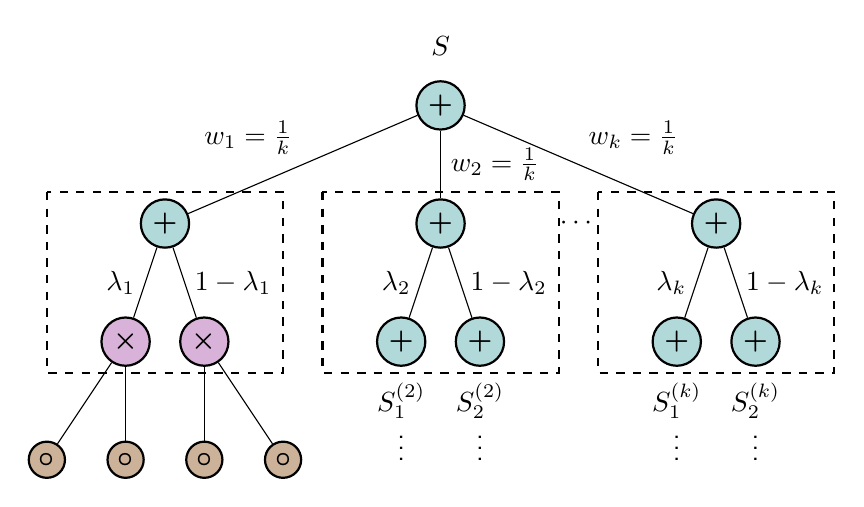
\begin{tikzpicture}[every node/.style={thick}]
       \newSumNode{r}{0,0};
       \newSumNode{s1}{-3.5,-1.5};
       \newSumNode{s2}{0.0,-1.5};
       \node (si) at (1.75, -1.5) {$\cdots$};
       \newSumNode{sk}{3.5,-1.5};
       \newProdNode{s11}{$(s1) + (-0.5,-1.5)$};
       \newProdNode{s12}{$(s1) + (+0.5,-1.5)$};
       \newSumNode{s21}{$(s2) + (-0.5,-1.5)$};
       \newSumNode{s22}{$(s2) + (+0.5,-1.5)$};
       \newSumNode{sk1}{$(sk) + (-0.5,-1.5)$};
       \newSumNode{sk2}{$(sk) + (+0.5,-1.5)$};

       \newLeafNode{l1p}{$(s11) + (-1.0,-1.5)$};
       \newLeafNode{l1n}{$(s11) + (+0.0,-1.5)$};
       \newLeafNode{l2p}{$(s12) + (-0.0,-1.5)$};
       \newLeafNode{l2n}{$(s12) + (+1.0,-1.5)$};

       \node at ($(r) + (0,0.75)$) {$S$};
       \node at ($(s21) + (0,-0.75)$) {$S_1^{(2)}$};
       \node at ($(s22) + (0,-0.75)$) {$S_2^{(2)}$};
       \node at ($(sk1) + (0,-0.75)$) {$S_1^{(k)}$};
       \node at ($(sk2) + (0,-0.75)$) {$S_2^{(k)}$};
       \node at ($(s21) + (0,-1.25)$) {$\vdots$};
       \node at ($(s22) + (0,-1.25)$) {$\vdots$};
       \node at ($(sk1) + (0,-1.25)$) {$\vdots$};
       \node at ($(sk2) + (0,-1.25)$) {$\vdots$};

       \draw (r) -- node[above left]{$w_1=\frac{1}{k}$} (s1);
       \draw (r) -- node[right]{$w_2=\frac{1}{k}$} (s2);
       \draw (r) -- node[above right]{$w_k=\frac{1}{k}$} (sk);
       \draw (s1) -- node[left]{$\lambda_1$} (s11);
       \draw (s2) -- node[left]{$\lambda_2$} (s21);
       \draw (sk) -- node[left]{$\lambda_k$} (sk1);
       \draw (s1) -- node[right]{$1-\lambda_1$} (s12);
       \draw (s2) -- node[right]{$1-\lambda_2$} (s22);
       \draw (sk) -- node[right]{$1-\lambda_k$} (sk2);

       \draw (s11) -- (l1p);
       \draw (s11) -- (l1n);
       \draw (s12) -- (l2p);
       \draw (s12) -- (l2n);

       \draw[thick,dashed] ($(s11) + (-1.0,1.9)$) rectangle ($(s12) + (1.0,-0.4)$);
       \draw[thick,dashed] ($(s21) + (-1.0,1.9)$) rectangle ($(s22) + (1.0,-0.4)$);
       \draw[thick,dashed] ($(sk1) + (-1.0,1.9)$) rectangle ($(sk2) + (1.0,-0.4)$);
     \end{tikzpicture}
   }
 \end{center}
\colorbox{pyellow}{\underline{Sum nodes as RPs:}}
\begin{center}
  \resizebox{0.55\textwidth}{!}{
  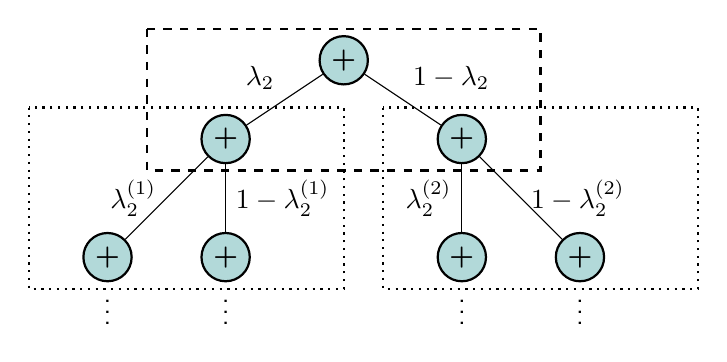
\begin{tikzpicture}[every node/.style={thick}]
   \newSumNode{r}{0.0,0.0};
   \newSumNode{s1}{$(r) + (-1.5,-1.0)$};
   \newSumNode{s2}{$(r) + (+1.5,-1.0)$};
   \newSumNode{s11}{$(s1) + (-1.5,-1.5)$};
   \newSumNode{s12}{$(s1) + (+0.0,-1.5)$};
   \newSumNode{s21}{$(s2) + (-0.0,-1.5)$};
   \newSumNode{s22}{$(s2) + (+1.5,-1.5)$};

   \draw (r) -- node[above left]{$\lambda_2$} (s1);
   \draw (r) -- node[above right]{$1-\lambda_2$} (s2);
   \draw (s1) -- node[left]{$\lambda_2^{(1)}$} (s11);
   \draw (s1) -- node[right]{$1-\lambda_2^{(1)}$} (s12);
   \draw (s2) -- node[left]{$\lambda_2^{(2)}$} (s21);
   \draw (s2) -- node[right]{$1-\lambda_2^{(2)}$} (s22);

   \node at ($(s11) + (0,-0.6)$) {$\vdots$};
   \node at ($(s12) + (0,-0.6)$) {$\vdots$};
   \node at ($(s21) + (0,-0.6)$) {$\vdots$};
   \node at ($(s22) + (0,-0.6)$) {$\vdots$};

   \draw[thick,dashed] ($(s1) + (-1.0,1.4)$) rectangle ($(s2) + (1.0,-0.4)$);
   \draw[thick,dotted] ($(s11) + (-1.0,1.9)$) rectangle ($(s12) + (1.5,-0.4)$);
   \draw[thick,dotted] ($(s21) + (-1.0,1.9)$) rectangle ($(s22) + (1.5,-0.4)$);
 \end{tikzpicture}
 }
\end{center}
\colorbox{pyellow}{\underline{Mixtures of RPs:}}
\begin{center}
  \resizebox{0.45\textwidth}{!}{
  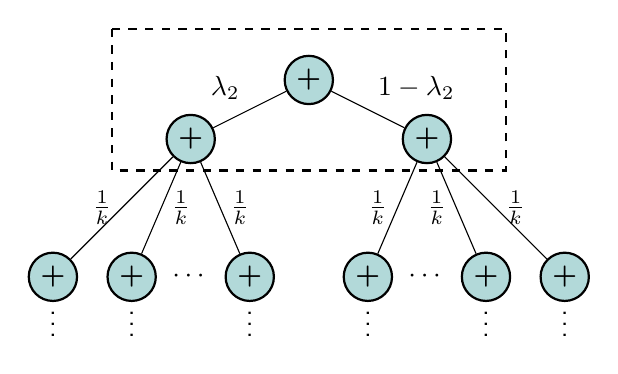
\begin{tikzpicture}[every node/.style={thick}]
    \newSumNode{r}{0.0,-0.0};
     \newSumNode{s1}{$(r) + (-1.5,-0.75)$};
     \newSumNode{s2}{$(r) + (+1.5,-0.75)$};
     \newSumNode{s11}{$(s1) + (-1.75,-1.75)$};
     \newSumNode{s12}{$(s1) + (-0.75,-1.75)$};
     \node at ($(s12)+(0.75,0)$) {$\cdots$};
     \newSumNode{s13}{$(s1) + (0.75,-1.75)$};
     \newSumNode{s21}{$(s2) + (-0.75,-1.75)$};
     \node at ($(s21)+(0.75,0)$) {$\cdots$};
     \newSumNode{s22}{$(s2) + (+0.75,-1.75)$};
     \newSumNode{s23}{$(s2) + (+1.75,-1.75)$};

     \node at ($(s11) + (0,-0.5)$) {$\vdots$};
     \node at ($(s12) + (0,-0.5)$) {$\vdots$};
     \node at ($(s13) + (0,-0.5)$) {$\vdots$};
     \node at ($(s21) + (0,-0.5)$) {$\vdots$};
     \node at ($(s22) + (0,-0.5)$) {$\vdots$};
     \node at ($(s23) + (0,-0.5)$) {$\vdots$};

     \draw (r) -- node[above left]{$\lambda_2$} (s1);
     \draw (r) -- node[above right]{$1-\lambda_2$} (s2);
     \draw (s1) -- node[ left]{$\frac{1}{k}$} (s11);
     \draw (s1) -- node[right]{$\frac{1}{k}$} (s12);
     \draw (s1) -- node[right]{$\frac{1}{k}$} (s13);
     \draw (s2) -- node[left]{$\frac{1}{k}$} (s21);
     \draw (s2) -- node[left]{$\frac{1}{k}$} (s22);
     \draw (s2) -- node[ right]{$\frac{1}{k}$} (s23);

     \draw[thick,dashed] ($(s1) + (-1.0,1.4)$) rectangle ($(s2) + (1.0,-0.4)$);
   \end{tikzpicture}
 }
\end{center}
\end{minipage}

\blankpage

\begin{minipage}{0.495\textwidth}

\begin{center}
\begin{tikzpicture}
\begin{axis}
\addplot [only marks,opacity=0.5] table {data/moons.data};
\end{axis}
\end{tikzpicture}
\end{center}
\vskip 1.5cm
\begin{center}
\begin{tabular}{c|r|rrrr}
  \hline %{2-6}
  \textbf{EM} &\textbf{$\sigma^2 \geq$} & \textbf{RPMaxS} & \textbf{RPMax} & \textbf{RPSIDS} & \textbf{RPSID} \\
  \hline
  \multirow{4}{*}{\textbf{Batch}} & fixed & -1.083 & -1.139 & -1.106 & -1.074 \\
  & 0.10 & -1.616 & -1.616 & -1.616 & -1.616 \\
  & 0.05 & -1.387 & -1.388 & -1.387 & -1.385 \\
  & 0.01 & -1.034 & -1.041 & -1.035 & -1.032 \\
  \hline
  \multirow{4}{*}{\textbf{Online}} & fixed & -1.089 & -1.119 & -1.080 & -1.108 \\
  & 0.10 & -1.623 & -1.627 & -1.624 & -1.637 \\
  & 0.05 & -1.416 & -1.402 & -1.408 & -1.412 \\
  & 0.01 & -1.139 & -1.080 & -1.114 & -1.105 \\ 
  \hline
\end{tabular}
\end{center}
\end{minipage}
\begin{minipage}{0.495\textwidth}
  \vskip 0.5cm
\begin{center}
\resizebox{\textwidth}{!}{
\begin{tabular}{c|ccccc}
  & & fixed & 0.1 & 0.05 & 0.01 \\
  & & & & &\\
  \multirow{4}{*}[-0.75cm]{\rotatebox{90}{\Large\textsc{Batch}}} & \multirow{2}{*}[0.5cm]{\rotatebox{90}{\Large\textsc{RPSID}}}
  &
  \includegraphics[width=0.245\textwidth]{figures/nogauss_moons_sid.pdf}
  &
  \includegraphics[width=0.245\textwidth]{figures/gauss01_moons_sid.pdf}
  &
  \includegraphics[width=0.245\textwidth]{figures/gauss005_moons_sid.pdf}
  &
  \includegraphics[width=0.245\textwidth]{figures/gauss001_moons_sid.pdf}\\
  & &
  \includegraphics[width=0.245\textwidth]{figures/nogauss_moons_density_sid.pdf}
  &
  \includegraphics[width=0.245\textwidth]{figures/gauss01_moons_density_sid.pdf}
  &
  \includegraphics[width=0.245\textwidth]{figures/gauss005_moons_density_sid.pdf}
  &
  \includegraphics[width=0.245\textwidth]{figures/gauss001_moons_density_sid.pdf}\\
  & \multirow{2}{*}[0.75cm]{\rotatebox[origin=c]{90}{\Large\textsc{RPMAX}}}
  &
  \includegraphics[width=0.245\textwidth]{figures/nogauss_moons_max.pdf}
  &
  \includegraphics[width=0.245\textwidth]{figures/gauss01_moons_max.pdf}
  &
  \includegraphics[width=0.245\textwidth]{figures/gauss005_moons_max.pdf}
  &
  \includegraphics[width=0.245\textwidth]{figures/gauss001_moons_max.pdf}\\
  & &
  \includegraphics[width=0.245\textwidth]{figures/nogauss_moons_density_max.pdf}
  &
  \includegraphics[width=0.245\textwidth]{figures/gauss01_moons_density_max.pdf}
  &
  \includegraphics[width=0.245\textwidth]{figures/gauss005_moons_density_max.pdf}
  &
  \includegraphics[width=0.245\textwidth]{figures/gauss001_moons_density_max.pdf}\\
  & & & & &\\
  \hline
  & & & & &\\
  \multirow{4}{*}[-0.75cm]{\rotatebox{90}{\Large\textsc{Online}}} & \multirow{2}{*}[0.5cm]{\rotatebox{90}{\Large\textsc{RPSID}}}
  & \includegraphics[width=0.245\textwidth]{figures/online_nogauss_moons_sid.pdf} &
  \includegraphics[width=0.245\textwidth]{figures/online_gauss01_moons_sid.pdf} &
  \includegraphics[width=0.245\textwidth]{figures/online_gauss005_moons_sid.pdf} &
  \includegraphics[width=0.245\textwidth]{figures/online_gauss001_moons_sid.pdf}\\
                                                                                 & &
  \includegraphics[width=0.245\textwidth]{figures/online_nogauss_moons_density_sid.pdf} &
  \includegraphics[width=0.245\textwidth]{figures/online_gauss01_moons_density_sid.pdf} &
  \includegraphics[width=0.245\textwidth]{figures/online_gauss005_moons_density_sid.pdf} &
  \includegraphics[width=0.245\textwidth]{figures/online_gauss001_moons_density_sid.pdf}\\
  & \multirow{2}{*}[0.75cm]{\rotatebox{90}{\Large\textsc{RPMAX}}}
  &
  \includegraphics[width=0.245\textwidth]{figures/online_nogauss_moons_max.pdf} &
  \includegraphics[width=0.245\textwidth]{figures/online_gauss01_moons_max.pdf} &
  \includegraphics[width=0.245\textwidth]{figures/online_gauss005_moons_max.pdf} &
  \includegraphics[width=0.245\textwidth]{figures/online_gauss001_moons_max.pdf}\\
                                                                                 & &
  \includegraphics[width=0.245\textwidth]{figures/online_nogauss_moons_density_max.pdf} &
  \includegraphics[width=0.245\textwidth]{figures/online_gauss01_moons_density_max.pdf} &
  \includegraphics[width=0.245\textwidth]{figures/online_gauss005_moons_density_max.pdf} &
  \includegraphics[width=0.245\textwidth]{figures/online_gauss001_moons_density_max.pdf}
\end{tabular}
}
\end{center}
\end{minipage}

\begin{center}
\begin{minipage}{0.45\textwidth}
\colorbox{pyellow}{\underline{Experiments:}}
\begin{itemize}\itemsep0pt
  \item Synthetic dataset: \texttt{2-moons};
  \item Benchmark datasets: 20 binary density datasets;
  \item Almost never best, but promising results given its simplicity.
\end{itemize}
\end{minipage}~\begin{minipage}{0.45\textwidth}
\vskip 0.5cm
\colorbox{pyellow}{\underline{Further work:}}
\begin{itemize}\itemsep0pt
  \item RP theoretical guarantees extend to PCs?
  \item Are there other desirable statistical properties?
  \item RPs in more elaborate structural learners?
  \item More complex leaf distributions (CLTs, other PCs)?
\end{itemize}
\end{minipage}
\end{center}

\vskip 0.5cm
\hspace{2cm}\textcolor{gray}{\cite{gens13,mei20,liang17,dimauro21}}
\vskip 1.0cm

\resizebox{\textwidth}{!}{
\begin{tabular}{l|rrrr|rrrr|rrrr}
\hline
\textbf{Dataset} & \textbf{RPMaxSD} & \textbf{RPMaxD} & \textbf{RPSIDSD} & \textbf{RPSIDD} & \textbf{RPMaxS} & \textbf{RPMax} & \textbf{RPSIDS} & \textbf{RPSID} & \textbf{LSPN} & \textbf{Strudel} & \textbf{LPSDD} & \textbf{EXPC}\\
\hline
%\textsc{accidents } &   -36.77 &  -36.67 &  -36.96 &  -36.47 &  -37.41 &  -37.48 &  -37.16 &  -37.39 & \underline{-30.03} & \textbf{-28.73} & $|$-30.16$|$ &  -31.02\\
%\textsc{ad        } &   -36.58 &  -36.19 &  -36.14 &  -35.88 &  -33.40 &  -32.83 &  -34.42 &  -35.55 & $|$-19.73$|$ & \underline{-16.38} &  -31.78 & \textbf{-15.50}\\
%\textsc{audio     } &   -40.25 &  -40.25 & $|$-40.20$|$ & \underline{-40.20} &  -40.29 &  -40.25 &  -40.28 &  -40.23 &  -40.50 &  -41.50 & \textbf{-39.94} &  -40.91\\
%\textsc{bbc       } &  -253.15 & $|$-251.71$|$ & -252.48 & -252.65 & -254.71 & -254.57 & -254.74 & -254.99 & \underline{-250.68} & -254.41 & -253.19 & \textbf{-248.34}\\
%\textsc{netflix   } &   -57.20 &  -57.21 &  -57.22 & \underline{-56.89} &  -57.53 &  -57.40 &  -57.45 &  -57.44 & $|$-57.02$|$ &  -58.69 & \textbf{-55.71} &  -57.58\\
%\textsc{book      } &  -34.84 &  -34.92 &  -34.87 &  -34.82 & $|$-34.75$|$ &  -34.85 & \underline{-34.74} & \textbf{-34.66} &  -35.88 &  -34.99 &  -34.97 &  -34.75\\
%\textsc{20-newsgrp} &  -154.20 & -154.58 & $|$-153.91$|$ & \textbf{-153.51} & -155.39 & -155.41 & -155.59 & -156.08 & -155.92 & -154.47 & -155.97 & \underline{-153.75}\\
%\textsc{reuters-52} &  -87.01 &  -86.70 &  -86.79 &  -86.56 &  -87.58 &  -87.23 &  -86.33 &  -87.28 & \underline{-85.06} & $|$-86.22$|$ &  -89.61 & \textbf{-84.70}\\
%\textsc{webkb     } & -157.49 & -157.66 & $|$-157.06$|$ & -157.07 & -158.46 & -158.72 & -158.07 & -157.94 & -158.20 & \underline{-155.33} & -161.09 & \textbf{-153.67}\\
%\textsc{dna       } &  -97.89 &  -96.86 &  -97.28 &  -97.64 &  -97.45 &  -97.17 &  -97.47 &  -96.68 & \textbf{-82.52} & \underline{-86.22} &  -88.01 & $|$-86.61$|$\\
%\textsc{jester    } & $|$-53.05$|$ & \underline{-52.99} &  -53.09 &  -53.05 &  -53.21 &  -53.24 &  -53.13 &  -53.06 &  -75.98 &  -55.03 & \textbf{-51.29} &  -53.43\\
%\textsc{kdd       } &    -2.17 &   -2.18 &   -2.17 &   -2.18 &   -2.16 &   -2.16 &   -2.16 &   -2.17 &   -2.18 & \underline{-2.13} & \textbf{-2.11} & $|$-2.15$|$\\
%\textsc{kosarek   } &   -11.11 &  -11.14 &  -11.14 &  -11.15 &  -11.06 &  -11.07 &  -11.02 &  -11.08 &  -10.98 & \underline{-10.68} & \textbf{-10.52} & $|$-10.77$|$\\
%\textsc{msnbc     } &    -6.24 &   -6.24 &   -6.25 &   -6.32 &   -6.18 &   -6.18 &   -6.20 &   -6.28 & $|$-6.11$|$ & \textbf{-6.04} & \underline{-6.04} &   -6.18\\
%\textsc{msweb     } &   -10.51 &  -10.55 &  -10.53 &  -10.59 &  -10.25 &  -10.26 &  -10.25 &  -10.29 &  -10.25 & \textbf{-9.71} & \underline{-9.89} & $|$-9.93$|$\\
%\textsc{nltcs     } &   -6.02 &   -6.02 &   -6.03 &   -6.05 & $|$-6.01$|$ & \underline{-6.01} &   -6.01 &   -6.01 &   -6.11 &   -6.06 & \textbf{-5.99} &   -6.05\\
%\textsc{plants    } &  -13.94 &  -14.06 &  -14.00 &  -13.96 &  -14.07 &  -13.86 &  -14.02 &  -13.94 & \textbf{-12.97} & \underline{-12.98} & $|$-13.02$|$ &  -14.19\\
%\textsc{pumsb-star} &   -33.53 &  -34.23 &  -33.55 &  -32.73 &  -34.35 &  -34.24 &  -34.53 &  -33.92 & \underline{-24.78} & \textbf{-24.12} &  -26.12 & $|$-26.06$|$\\
%\textsc{eachmovie } &  -53.03 & $|$-52.93$|$ &  -52.94 &  -52.96 &  -53.03 &  -53.28 & \underline{-52.88} &  -53.15 & \textbf{-52.48} &  -53.67 &  -58.01 &  -54.82\\
%\textsc{retail    } &   -11.02 &  -11.00 &  -11.01 &  -11.03 & $|$-10.93$|$ &  -10.93 &  -10.94 &  -10.93 &  -11.04 & \underline{-10.81} & \textbf{-10.72} &  -10.94\\
\textsc{nltcs     } &   -6.02 &   -6.02 &   -6.03 &   -6.05 & $|$-6.01$|$ & \underline{-6.01} &   -6.01 &   -6.01 &   -6.11 &   -6.06 & \textbf{-5.99} &   -6.05\\
\textsc{plants    } &  -13.94 &  -14.06 &  -14.00 &  -13.96 &  -14.07 &  -13.86 &  -14.02 &  -13.94 & \textbf{-12.97} & \underline{-12.98} & $|$-13.02$|$ &  -14.19\\
\textsc{audio     } &   -40.25 &  -40.25 & $|$-40.20$|$ & \underline{-40.20} &  -40.29 &  -40.25 &  -40.28 &  -40.23 &  -40.50 &  -41.50 & \textbf{-39.94} &  -40.91\\
\textsc{jester    } & $|$-53.05$|$ & \underline{-52.99} &  -53.09 &  -53.05 &  -53.21 &  -53.24 &  -53.13 &  -53.06 &  -75.98 &  -55.03 & \textbf{-51.29} &  -53.43\\
\textsc{netflix   } &   -57.20 &  -57.21 &  -57.22 & \underline{-56.89} &  -57.53 &  -57.40 &  -57.45 &  -57.44 & $|$-57.02$|$ &  -58.69 & \textbf{-55.71} &  -57.58\\
\textsc{accidents } &   -36.77 &  -36.67 &  -36.96 &  -36.47 &  -37.41 &  -37.48 &  -37.16 &  -37.39 & \underline{-30.03} & \textbf{-28.73} & $|$-30.16$|$ &  -31.02\\
\textsc{book      } &  -34.84 &  -34.92 &  -34.87 &  -34.82 & $|$-34.75$|$ &  -34.85 & \underline{-34.74} & \textbf{-34.66} &  -35.88 &  -34.99 &  -34.97 &  -34.75\\
\textsc{dna       } &  -97.89 &  -96.86 &  -97.28 &  -97.64 &  -97.45 &  -97.17 &  -97.47 &  -96.68 & \textbf{-82.52} & \underline{-86.22} &  -88.01 & $|$-86.61$|$\\
\hline
\textsc{nltcs     } &   3s &   2s &   5s &   3s &   3s &   2s &   6s &   3s & 7m & 3m & 6m & -- \\
\textsc{plants    } &   8s &   4s &  12s &   7s &   7s &   4s &  12s &   7s & 50m & 41m & 26m & -- \\
\textsc{audio     } &   9s &   4s &  14s &   8s &   8s &   4s &  14s &   8s & 2h & 33m & 51m & -- \\
\textsc{jester    } &   5s &   3s &   9s &   5s &   4s &   3s &   9s &   5s & 52m & 24m & 37m & -- \\
\textsc{netflix   } &   8s &   4s &  15s &   8s &   7s &   4s &  14s &   8s & 1h & 14m & 33m & -- \\
\textsc{accidents } &   7s &   4s &  13s &   7s &   7s &   4s &  13s &   7s & 47m & 20m & 41m & -- \\
\textsc{book      } &  12s &   6s &  18s &  10s &   9s &   6s &  17s &  10s & $>$3h & 8m & 1.3h & -- \\
\textsc{dna       } &   1s &   1s &   3s &   2s &   2s &   1s &   2s &   1s & $>$3h & $>$3h & $>$3h & -- \\
\hline
  \end{tabular}
}

% Title
%\blankpage

%\begin{center}
  %\vspace*{\fill}
  %\vskip 0.75cm
  %\resizebox{\textwidth}{!}{
    %\begin{minipage}{0.375\textwidth}
      %\begin{center}
        %\textcolor{pdblue}{\textbf{Fast and Accurate Learning of\\Probabilistic Circuits by Random
        %Projections}}
      %\end{center}
    %\end{minipage}
  %}
  %\vskip 1.5cm
  %\resizebox{0.8\textwidth}{!}{
    %\begin{minipage}{0.25\textwidth}
      %\begin{center}
        %\textcolor{pdblue}{\textbf{Renato L. Geh}}

        %\texttt{renatolg@ime.usp.br}
      %\end{center}
    %\end{minipage}\hspace{-1cm}\begin{minipage}{0.25\textwidth}
      %\begin{center}
        %\textcolor{pdblue}{Denis D. Mauá}

        %\texttt{ddm@ime.usp.br}
      %\end{center}
    %\end{minipage}
  %}
  %\vskip 1.5cm
  %\resizebox{0.9\textwidth}{!}{
  %\begin{minipage}{0.5\textwidth}
    %\color{ppurple}
    %\begin{center}
      %Department of Computer Science
    %\end{center}
    %\begin{center}
      %Institute of Mathematics and Statistics, University of São Paulo
    %\end{center}
  %\end{minipage}
  %}
  %\vskip 1cm
  %\begin{center}
    %\includegraphics[width=3cm]{figures/usp.eps}
  %\end{center}
  %\vskip 0.5cm
  %\resizebox{\textwidth}{!}{
    %\begin{minipage}{0.5\textwidth}
      %\begin{center}
        %\color{pbrickred}\textbf{TPM 2021}
      %\end{center}
    %\end{minipage}
  %}
  %\vspace*{\fill}
%\end{center}

%% Random Projections
%\newpage

%\resizebox{0.4\textwidth}{!}{\textcolor{pdblue}{Random Projections}}

%\resizebox{0.495\textwidth}{!}{
%\begin{minipage}{0.39\textwidth}
%\colorbox{pyellow}{\underline{\cite{correia20}: there is a link between DTs and PCs!}}

%\begin{itemize}\itemsep0pt
  %\item Well known, established results in DTs;
  %\item But mostly in supervised tasks; \textcolor{gray}{\cite{khosravi20}}
  %\item What if we explore this link in an unsupervised context?
%\end{itemize}

%\colorbox{pyellow}{\underline{Random Projections (RPs):}}

%\begin{itemize}\itemsep0pt
  %\item Axis-aligned projections (kd-trees) are not good enough;
  %\item Splitting by the median is not good enough;
  %\item What about \textbf{random projections}?
%\end{itemize}

%\begin{center}
  %\colorbox{pteal!50}{\cite{rpmax} showed that it is!}
%\end{center}
%\vskip 0.3cm

%\colorbox{pyellow}{\underline{Idea behind RPs:}}

%\begin{itemize}\itemsep0pt
  %\item Sample random direction $u$;
  %\item Construct hyperplane $\mathcal{H}$ with $u$;
  %\item Apply perturbation $\delta$ to $\mathcal{H}$ st. divides data somewhat equally;
  %\item Choice of $\delta$:
    %\begin{description}\itemsep0pt
      %\item[\textsc{Max}:] by diameter (maximal distance);
      %\item[\textsc{SID}:] by Square Interpoint Distance.
    %\end{description}
%\end{itemize}

%\end{minipage}}\resizebox{0.495\textwidth}{!}{\begin{minipage}{0.36\textwidth}
%\resizebox{\textwidth}{!}{\begin{tikzpicture}
  %\node[rotate=90] at (-2,0) {\large\textsc{Median}};
  %\node at (0.75,0) {\includegraphics[width=0.49\textwidth]{figures/median_1.pdf}};
  %\node at (5.75,0) {\includegraphics[width=0.49\textwidth]{figures/median_2.pdf}};
  %\node[rotate=90] at (-2,-3.5) {\large\textsc{Max}};
  %\node at (0.75,-3.5) {\includegraphics[width=0.49\textwidth]{figures/max_1.pdf}};
  %\node at (5.75,-3.5) {\includegraphics[width=0.49\textwidth]{figures/max_2.pdf}};
  %\node[rotate=90] at (-2,-7.0) {\large\textsc{SID}};
  %\node at (0.75,-7.0) {\includegraphics[width=0.49\textwidth]{figures/sid_1.pdf}};
  %\node at (5.75,-7.0) {\includegraphics[width=0.49\textwidth]{figures/sid_2.pdf}};
%\end{tikzpicture}}
%\end{minipage}}

%% LearnRP 1

%\newpage
%\resizebox{0.8\textwidth}{!}{\textcolor{pdblue}{Learning Probabilistic Circuits by Random Projections}}

%\resizebox{0.495\textwidth}{!}{
%\begin{minipage}{0.39\textwidth}

%\colorbox{pyellow}{\underline{Sum nodes as RPs:}}
%\begin{itemize}\itemsep0pt
  %\item Directly translate RP Decision Trees to PCs;
  %\item Projections define a clustering of data;
  %\item LearnSPN-like on sums;
  %\item Eventually learn a leaf distribution:
    %\begin{enumerate}[label=(\roman*)]\itemsep0pt
      %\item Fully factorized circuit;
      %\item RAT-SPN (\cite{peharz19}).
    %\end{enumerate}
%\end{itemize}
%\vskip -0.25cm
%\begin{algorithm}[H]
  %\rmfamily
  %\caption*{\textproc{\rmfamily LearnRP-S}}\label{alg:learnrp-single}
  %\begin{algorithmic}[1]
    %\Require Dataset $S\subset\mathbb{R}^n$, no.\ of trials $t$, no.\ of trees $k$
    %\Ensure A probabilistic circuit
    %\If{it is the first recursion}
      %\State \textbf{return} $\sum_{i=1}^k \frac{1}{k}\textproc{LearnRP-S}(S, t, k)$
    %\Else
      %\State Sample $t$ RPs by some criteria
      %\State Select split ($S_1$,$S_2$) that minimizes the avg. diam. of $S$
      %%\State Call such split $S_1$, $S_2$
      %\If{$|S_1|$ is small} \ $P_1\gets\textproc{LearnDistribution}(S_1)$
      %\Else \ $P_1\gets\textproc{LearnRP-S}(S_1, t, k)$ \EndIf
      %\If{$|S_2|$ is small} \ $P_2\gets \textproc{LearnDistribution}(S_2)$
      %\Else  \ $P_2\gets\textproc{LearnRP-S}(S_2, t, k)$ \EndIf
      %\State Set $\lambda \gets |S_1|/|S|$
      %\State \textbf{return} $\lambda\cdot P_1+(1-\lambda)\cdot P_2$
    %\EndIf
  %\end{algorithmic}
%\end{algorithm}
%\end{minipage}}\resizebox{0.5\textwidth}{!}{\begin{minipage}{0.35\textwidth}
  %\resizebox{\textwidth}{!}{
    %\begin{tikzpicture}[every node/.style={thick}]
       %\newSumNode{r}{0,0};
       %\newSumNode{s1}{-3.5,-1.5};
       %\newSumNode{s2}{0.0,-1.5};
       %\node (si) at (1.75, -1.5) {$\cdots$};
       %\newSumNode{sk}{3.5,-1.5};
       %\newProdNode{s11}{$(s1) + (-0.5,-1.5)$};
       %\newProdNode{s12}{$(s1) + (+0.5,-1.5)$};
       %\newSumNode{s21}{$(s2) + (-0.5,-1.5)$};
       %\newSumNode{s22}{$(s2) + (+0.5,-1.5)$};
       %\newSumNode{sk1}{$(sk) + (-0.5,-1.5)$};
       %\newSumNode{sk2}{$(sk) + (+0.5,-1.5)$};

       %\newLeafNode{l1p}{$(s11) + (-1.0,-1.5)$};
       %\newLeafNode{l1n}{$(s11) + (+0.0,-1.5)$};
       %\newLeafNode{l2p}{$(s12) + (-0.0,-1.5)$};
       %\newLeafNode{l2n}{$(s12) + (+1.0,-1.5)$};

       %\node at ($(r) + (0,0.75)$) {$S$};
       %\node at ($(s21) + (0,-0.75)$) {$S_1^{(2)}$};
       %\node at ($(s22) + (0,-0.75)$) {$S_2^{(2)}$};
       %\node at ($(sk1) + (0,-0.75)$) {$S_1^{(k)}$};
       %\node at ($(sk2) + (0,-0.75)$) {$S_2^{(k)}$};
       %\node at ($(s21) + (0,-1.25)$) {$\vdots$};
       %\node at ($(s22) + (0,-1.25)$) {$\vdots$};
       %\node at ($(sk1) + (0,-1.25)$) {$\vdots$};
       %\node at ($(sk2) + (0,-1.25)$) {$\vdots$};

       %\draw (r) -- node[above left]{$w_1=\frac{1}{k}$} (s1);
       %\draw (r) -- node[right]{$w_2=\frac{1}{k}$} (s2);
       %\draw (r) -- node[above right]{$w_k=\frac{1}{k}$} (sk);
       %\draw (s1) -- node[left]{$\lambda_1$} (s11);
       %\draw (s2) -- node[left]{$\lambda_2$} (s21);
       %\draw (sk) -- node[left]{$\lambda_k$} (sk1);
       %\draw (s1) -- node[right]{$1-\lambda_1$} (s12);
       %\draw (s2) -- node[right]{$1-\lambda_2$} (s22);
       %\draw (sk) -- node[right]{$1-\lambda_k$} (sk2);

       %\draw (s11) -- (l1p);
       %\draw (s11) -- (l1n);
       %\draw (s12) -- (l2p);
       %\draw (s12) -- (l2n);

       %\draw[thick,dashed] ($(s11) + (-1.0,1.9)$) rectangle ($(s12) + (1.0,-0.4)$);
       %\draw[thick,dashed] ($(s21) + (-1.0,1.9)$) rectangle ($(s22) + (1.0,-0.4)$);
       %\draw[thick,dashed] ($(sk1) + (-1.0,1.9)$) rectangle ($(sk2) + (1.0,-0.4)$);

       %\newSumNode{r}{0.0,-6};
       %\newSumNode{s1}{$(r) + (-1.5,-1.0)$};
       %\newSumNode{s2}{$(r) + (+1.5,-1.0)$};
       %\newSumNode{s11}{$(s1) + (-1.5,-1.5)$};
       %\newSumNode{s12}{$(s1) + (+0.0,-1.5)$};
       %\newSumNode{s21}{$(s2) + (-0.0,-1.5)$};
       %\newSumNode{s22}{$(s2) + (+1.5,-1.5)$};

       %\draw (r) -- node[above left]{$\lambda_2$} (s1);
       %\draw (r) -- node[above right]{$1-\lambda_2$} (s2);
       %\draw (s1) -- node[left]{$\lambda_2^{(1)}$} (s11);
       %\draw (s1) -- node[right]{$1-\lambda_2^{(1)}$} (s12);
       %\draw (s2) -- node[left]{$\lambda_2^{(2)}$} (s21);
       %\draw (s2) -- node[right]{$1-\lambda_2^{(2)}$} (s22);

       %\node at ($(s11) + (0,-0.6)$) {$\vdots$};
       %\node at ($(s12) + (0,-0.6)$) {$\vdots$};
       %\node at ($(s21) + (0,-0.6)$) {$\vdots$};
       %\node at ($(s22) + (0,-0.6)$) {$\vdots$};

       %\draw[thick,dashed] ($(s1) + (-1.0,1.4)$) rectangle ($(s2) + (1.0,-0.4)$);
       %\draw[thick,dotted] ($(s11) + (-1.0,1.9)$) rectangle ($(s12) + (1.5,-0.4)$);
       %\draw[thick,dotted] ($(s21) + (-1.0,1.9)$) rectangle ($(s22) + (1.5,-0.4)$);
     %\end{tikzpicture}
   %}
%\end{minipage}}

%% LearnRP 2
%\newpage
%\resizebox{0.8\textwidth}{!}{\textcolor{pdblue}{Learning Probabilistic Circuits by Random Projections}}

%\resizebox{0.495\textwidth}{!}{
%\begin{minipage}{0.39\textwidth}

%\colorbox{pyellow}{\underline{Mixtures of RPs:}}

%\begin{itemize}\itemsep0pt
  %\item Same as before, but now with $k$ projections;
  %\item At each data split, creates a ``mixture node'';
  %\item Children are projections.
%\end{itemize}
%\vskip -0.25cm
%\begin{algorithm}[H]
  %\rmfamily
  %\caption*{\textproc{LearnRP}}\label{alg:learnrp}
  %\begin{algorithmic}[1]
    %\Require Dataset $S\subset\mathbb{R}^n$, no. of trials $t$, no. of mixtures $k$
    %\Ensure A probabilistic circuit
    %\For{$i=1,\dotsc,k$}
      %\State Sample $t$ splits by some criteria
      %\State Select split $(S_1,S_2)$ that minimizes the avg. diam. of $S$
      %%\State Call such split $S_1$, $S_2$
      %\If{$|S_1|$ is small} \State $P_1\gets\textproc{LearnDistribution}(S_1)$
      %\Else \ $P_1\gets\textproc{LearnRP}(S_1, t, k)$ \EndIf
      %\If{$|S_2|$ is small} \State $P_2\gets\textproc{LearnDistribution}(S_2)$
      %\Else \ $P_2\gets\textproc{LearnRP}(S_2, t, k)$ \EndIf
      %\State Set $\lambda \gets |S_1|/|S|$
      %\State Compute $C_i \gets \lambda\cdot P_1+(1-\lambda)\cdot P_2$
    %\EndFor
    %\State \textbf{return} $\sum_{i=1}^k \frac{1}{k} C_i$
  %\end{algorithmic}
%\end{algorithm}

%\end{minipage}}\resizebox{0.5\textwidth}{!}{\begin{minipage}{0.35\textwidth}
  %\resizebox{\textwidth}{!}{
    %\begin{tikzpicture}[every node/.style={thick}]
       %\newSumNode{r}{0,0};
       %\newSumNode{s1}{-3.5,-1.5};
       %\newSumNode{s2}{0.0,-1.5};
       %\node (si) at (1.75, -1.5) {$\cdots$};
       %\newSumNode{sk}{3.5,-1.5};
       %\newProdNode{s11}{$(s1) + (-0.5,-1.5)$};
       %\newProdNode{s12}{$(s1) + (+0.5,-1.5)$};
       %\newSumNode{s21}{$(s2) + (-0.5,-1.5)$};
       %\newSumNode{s22}{$(s2) + (+0.5,-1.5)$};
       %\newSumNode{sk1}{$(sk) + (-0.5,-1.5)$};
       %\newSumNode{sk2}{$(sk) + (+0.5,-1.5)$};

       %\newLeafNode{l1p}{$(s11) + (-1.0,-1.5)$};
       %\newLeafNode{l1n}{$(s11) + (+0.0,-1.5)$};
       %\newLeafNode{l2p}{$(s12) + (-0.0,-1.5)$};
       %\newLeafNode{l2n}{$(s12) + (+1.0,-1.5)$};

       %\node at ($(r) + (0,0.75)$) {$S$};
       %\node at ($(s21) + (0,-0.75)$) {$S_1^{(2)}$};
       %\node at ($(s22) + (0,-0.75)$) {$S_2^{(2)}$};
       %\node at ($(sk1) + (0,-0.75)$) {$S_1^{(k)}$};
       %\node at ($(sk2) + (0,-0.75)$) {$S_2^{(k)}$};
       %\node at ($(s21) + (0,-1.25)$) {$\vdots$};
       %\node at ($(s22) + (0,-1.25)$) {$\vdots$};
       %\node at ($(sk1) + (0,-1.25)$) {$\vdots$};
       %\node at ($(sk2) + (0,-1.25)$) {$\vdots$};

       %\draw (r) -- node[above left]{$w_1=\frac{1}{k}$} (s1);
       %\draw (r) -- node[right]{$w_2=\frac{1}{k}$} (s2);
       %\draw (r) -- node[above right]{$w_k=\frac{1}{k}$} (sk);
       %\draw (s1) -- node[left]{$\lambda_1$} (s11);
       %\draw (s2) -- node[left]{$\lambda_2$} (s21);
       %\draw (sk) -- node[left]{$\lambda_k$} (sk1);
       %\draw (s1) -- node[right]{$1-\lambda_1$} (s12);
       %\draw (s2) -- node[right]{$1-\lambda_2$} (s22);
       %\draw (sk) -- node[right]{$1-\lambda_k$} (sk2);

       %\draw (s11) -- (l1p);
       %\draw (s11) -- (l1n);
       %\draw (s12) -- (l2p);
       %\draw (s12) -- (l2n);

       %\draw[thick,dashed] ($(s11) + (-1.0,1.9)$) rectangle ($(s12) + (1.0,-0.4)$);
       %\draw[thick,dashed] ($(s21) + (-1.0,1.9)$) rectangle ($(s22) + (1.0,-0.4)$);
       %\draw[thick,dashed] ($(sk1) + (-1.0,1.9)$) rectangle ($(sk2) + (1.0,-0.4)$);

       %\newSumNode{r}{0.0,-6.0};
       %\newSumNode{s1}{$(r) + (-1.5,-0.75)$};
       %\newSumNode{s2}{$(r) + (+1.5,-0.75)$};
       %\newSumNode{s11}{$(s1) + (-1.75,-1.75)$};
       %\newSumNode{s12}{$(s1) + (-0.75,-1.75)$};
       %\node at ($(s12)+(0.75,0)$) {$\cdots$};
       %\newSumNode{s13}{$(s1) + (0.75,-1.75)$};
       %\newSumNode{s21}{$(s2) + (-0.75,-1.75)$};
       %\node at ($(s21)+(0.75,0)$) {$\cdots$};
       %\newSumNode{s22}{$(s2) + (+0.75,-1.75)$};
       %\newSumNode{s23}{$(s2) + (+1.75,-1.75)$};

       %\node at ($(s11) + (0,-0.5)$) {$\vdots$};
       %\node at ($(s12) + (0,-0.5)$) {$\vdots$};
       %\node at ($(s13) + (0,-0.5)$) {$\vdots$};
       %\node at ($(s21) + (0,-0.5)$) {$\vdots$};
       %\node at ($(s22) + (0,-0.5)$) {$\vdots$};
       %\node at ($(s23) + (0,-0.5)$) {$\vdots$};

       %\draw (r) -- node[above left]{$\lambda_2$} (s1);
       %\draw (r) -- node[above right]{$1-\lambda_2$} (s2);
       %\draw (s1) -- node[ left]{$\frac{1}{k}$} (s11);
       %\draw (s1) -- node[right]{$\frac{1}{k}$} (s12);
       %\draw (s1) -- node[right]{$\frac{1}{k}$} (s13);
       %\draw (s2) -- node[left]{$\frac{1}{k}$} (s21);
       %\draw (s2) -- node[left]{$\frac{1}{k}$} (s22);
       %\draw (s2) -- node[ right]{$\frac{1}{k}$} (s23);

       %\draw[thick,dashed] ($(s1) + (-1.0,1.4)$) rectangle ($(s2) + (1.0,-0.4)$);
     %\end{tikzpicture}
   %}
%\end{minipage}}

%% Experiments 1

%\newpage

%\resizebox{!}{0.75cm}{\textcolor{pdblue}{Experiments: \texttt{2-moons}}}

%\resizebox{0.495\textwidth}{!}{
%\begin{minipage}{0.39\textwidth}

%\begin{center}
%\begin{tikzpicture}
%\begin{axis}
%\addplot [only marks,opacity=0.5] table {data/moons.data};
%\end{axis}
%\end{tikzpicture}
%\vskip 1cm
%\begin{tabular}{c|r|rrrr}
  %\hline %{2-6}
  %\textbf{EM} &\textbf{$\sigma^2 \geq$} & \textbf{RPMaxS} & \textbf{RPMax} & \textbf{RPSIDS} & \textbf{RPSID} \\
  %\hline
  %\multirow{4}{*}{\textbf{Batch}} & fixed & -1.083 & -1.139 & -1.106 & -1.074 \\
  %& 0.10 & -1.616 & -1.616 & -1.616 & -1.616 \\
  %& 0.05 & -1.387 & -1.388 & -1.387 & -1.385 \\
  %& 0.01 & -1.034 & -1.041 & -1.035 & -1.032 \\
  %\hline
  %\multirow{4}{*}{\textbf{Online}} & fixed & -1.089 & -1.119 & -1.080 & -1.108 \\
  %& 0.10 & -1.623 & -1.627 & -1.624 & -1.637 \\
  %& 0.05 & -1.416 & -1.402 & -1.408 & -1.412 \\
  %& 0.01 & -1.139 & -1.080 & -1.114 & -1.105 \\ 
  %\hline
%\end{tabular}
%\end{center}

%\end{minipage}}\resizebox{0.5\textwidth}{!}{\begin{minipage}{0.35\textwidth}
%\begin{center}
%\resizebox{\textwidth}{!}{
%\begin{tabular}{c|ccccc}
  %& & fixed & 0.1 & 0.05 & 0.01 \\
  %& & & & &\\
  %\multirow{4}{*}[-0.75cm]{\rotatebox{90}{\Large\textsc{Batch}}} & \multirow{2}{*}[0.5cm]{\rotatebox{90}{\Large\textsc{RPSID}}}
  %&
  %\includegraphics[width=0.245\textwidth]{figures/nogauss_moons_sid.pdf}
  %&
  %\includegraphics[width=0.245\textwidth]{figures/gauss01_moons_sid.pdf}
  %&
  %\includegraphics[width=0.245\textwidth]{figures/gauss005_moons_sid.pdf}
  %&
  %\includegraphics[width=0.245\textwidth]{figures/gauss001_moons_sid.pdf}\\
  %& &
  %\includegraphics[width=0.245\textwidth]{figures/nogauss_moons_density_sid.pdf}
  %&
  %\includegraphics[width=0.245\textwidth]{figures/gauss01_moons_density_sid.pdf}
  %&
  %\includegraphics[width=0.245\textwidth]{figures/gauss005_moons_density_sid.pdf}
  %&
  %\includegraphics[width=0.245\textwidth]{figures/gauss001_moons_density_sid.pdf}\\
  %& \multirow{2}{*}[0.75cm]{\rotatebox[origin=c]{90}{\Large\textsc{RPMAX}}}
  %&
  %\includegraphics[width=0.245\textwidth]{figures/nogauss_moons_max.pdf}
  %&
  %\includegraphics[width=0.245\textwidth]{figures/gauss01_moons_max.pdf}
  %&
  %\includegraphics[width=0.245\textwidth]{figures/gauss005_moons_max.pdf}
  %&
  %\includegraphics[width=0.245\textwidth]{figures/gauss001_moons_max.pdf}\\
  %& &
  %\includegraphics[width=0.245\textwidth]{figures/nogauss_moons_density_max.pdf}
  %&
  %\includegraphics[width=0.245\textwidth]{figures/gauss01_moons_density_max.pdf}
  %&
  %\includegraphics[width=0.245\textwidth]{figures/gauss005_moons_density_max.pdf}
  %&
  %\includegraphics[width=0.245\textwidth]{figures/gauss001_moons_density_max.pdf}\\
  %& & & & &\\
  %\hline
  %& & & & &\\
  %\multirow{4}{*}[-0.75cm]{\rotatebox{90}{\Large\textsc{Online}}} & \multirow{2}{*}[0.5cm]{\rotatebox{90}{\Large\textsc{RPSID}}}
  %& \includegraphics[width=0.245\textwidth]{figures/online_nogauss_moons_sid.pdf} &
  %\includegraphics[width=0.245\textwidth]{figures/online_gauss01_moons_sid.pdf} &
  %\includegraphics[width=0.245\textwidth]{figures/online_gauss005_moons_sid.pdf} &
  %\includegraphics[width=0.245\textwidth]{figures/online_gauss001_moons_sid.pdf}\\
                                                                                 %& &
  %\includegraphics[width=0.245\textwidth]{figures/online_nogauss_moons_density_sid.pdf} &
  %\includegraphics[width=0.245\textwidth]{figures/online_gauss01_moons_density_sid.pdf} &
  %\includegraphics[width=0.245\textwidth]{figures/online_gauss005_moons_density_sid.pdf} &
  %\includegraphics[width=0.245\textwidth]{figures/online_gauss001_moons_density_sid.pdf}\\
  %& \multirow{2}{*}[0.75cm]{\rotatebox{90}{\Large\textsc{RPMAX}}}
  %&
  %\includegraphics[width=0.245\textwidth]{figures/online_nogauss_moons_max.pdf} &
  %\includegraphics[width=0.245\textwidth]{figures/online_gauss01_moons_max.pdf} &
  %\includegraphics[width=0.245\textwidth]{figures/online_gauss005_moons_max.pdf} &
  %\includegraphics[width=0.245\textwidth]{figures/online_gauss001_moons_max.pdf}\\
                                                                                 %& &
  %\includegraphics[width=0.245\textwidth]{figures/online_nogauss_moons_density_max.pdf} &
  %\includegraphics[width=0.245\textwidth]{figures/online_gauss01_moons_density_max.pdf} &
  %\includegraphics[width=0.245\textwidth]{figures/online_gauss005_moons_density_max.pdf} &
  %\includegraphics[width=0.245\textwidth]{figures/online_gauss001_moons_density_max.pdf}
%\end{tabular}
%}
%\end{center}
%\end{minipage}}

%\resizebox{!}{0.75cm}{\textcolor{pdblue}{Experiments: benchmark datasets}}

%\vskip 3cm

%\resizebox{\textwidth}{!}{
%\begin{tabular}{l|rrrr|rrrr|rrrr}
%\hline
%\textbf{Dataset} & \textbf{RPMaxSD} & \textbf{RPMaxD} & \textbf{RPSIDSD} & \textbf{RPSIDD} & \textbf{RPMaxS} & \textbf{RPMax} & \textbf{RPSIDS} & \textbf{RPSID} & \textbf{LSPN} & \textbf{Strudel} & \textbf{LPSDD} & \textbf{EXPC}\\
%\hline
%%\textsc{accidents } &   -36.77 &  -36.67 &  -36.96 &  -36.47 &  -37.41 &  -37.48 &  -37.16 &  -37.39 & \underline{-30.03} & \textbf{-28.73} & $|$-30.16$|$ &  -31.02\\
%%\textsc{ad        } &   -36.58 &  -36.19 &  -36.14 &  -35.88 &  -33.40 &  -32.83 &  -34.42 &  -35.55 & $|$-19.73$|$ & \underline{-16.38} &  -31.78 & \textbf{-15.50}\\
%%\textsc{audio     } &   -40.25 &  -40.25 & $|$-40.20$|$ & \underline{-40.20} &  -40.29 &  -40.25 &  -40.28 &  -40.23 &  -40.50 &  -41.50 & \textbf{-39.94} &  -40.91\\
%%\textsc{bbc       } &  -253.15 & $|$-251.71$|$ & -252.48 & -252.65 & -254.71 & -254.57 & -254.74 & -254.99 & \underline{-250.68} & -254.41 & -253.19 & \textbf{-248.34}\\
%%\textsc{netflix   } &   -57.20 &  -57.21 &  -57.22 & \underline{-56.89} &  -57.53 &  -57.40 &  -57.45 &  -57.44 & $|$-57.02$|$ &  -58.69 & \textbf{-55.71} &  -57.58\\
%%\textsc{book      } &  -34.84 &  -34.92 &  -34.87 &  -34.82 & $|$-34.75$|$ &  -34.85 & \underline{-34.74} & \textbf{-34.66} &  -35.88 &  -34.99 &  -34.97 &  -34.75\\
%%\textsc{20-newsgrp} &  -154.20 & -154.58 & $|$-153.91$|$ & \textbf{-153.51} & -155.39 & -155.41 & -155.59 & -156.08 & -155.92 & -154.47 & -155.97 & \underline{-153.75}\\
%%\textsc{reuters-52} &  -87.01 &  -86.70 &  -86.79 &  -86.56 &  -87.58 &  -87.23 &  -86.33 &  -87.28 & \underline{-85.06} & $|$-86.22$|$ &  -89.61 & \textbf{-84.70}\\
%%\textsc{webkb     } & -157.49 & -157.66 & $|$-157.06$|$ & -157.07 & -158.46 & -158.72 & -158.07 & -157.94 & -158.20 & \underline{-155.33} & -161.09 & \textbf{-153.67}\\
%%\textsc{dna       } &  -97.89 &  -96.86 &  -97.28 &  -97.64 &  -97.45 &  -97.17 &  -97.47 &  -96.68 & \textbf{-82.52} & \underline{-86.22} &  -88.01 & $|$-86.61$|$\\
%%\textsc{jester    } & $|$-53.05$|$ & \underline{-52.99} &  -53.09 &  -53.05 &  -53.21 &  -53.24 &  -53.13 &  -53.06 &  -75.98 &  -55.03 & \textbf{-51.29} &  -53.43\\
%%\textsc{kdd       } &    -2.17 &   -2.18 &   -2.17 &   -2.18 &   -2.16 &   -2.16 &   -2.16 &   -2.17 &   -2.18 & \underline{-2.13} & \textbf{-2.11} & $|$-2.15$|$\\
%%\textsc{kosarek   } &   -11.11 &  -11.14 &  -11.14 &  -11.15 &  -11.06 &  -11.07 &  -11.02 &  -11.08 &  -10.98 & \underline{-10.68} & \textbf{-10.52} & $|$-10.77$|$\\
%%\textsc{msnbc     } &    -6.24 &   -6.24 &   -6.25 &   -6.32 &   -6.18 &   -6.18 &   -6.20 &   -6.28 & $|$-6.11$|$ & \textbf{-6.04} & \underline{-6.04} &   -6.18\\
%%\textsc{msweb     } &   -10.51 &  -10.55 &  -10.53 &  -10.59 &  -10.25 &  -10.26 &  -10.25 &  -10.29 &  -10.25 & \textbf{-9.71} & \underline{-9.89} & $|$-9.93$|$\\
%%\textsc{nltcs     } &   -6.02 &   -6.02 &   -6.03 &   -6.05 & $|$-6.01$|$ & \underline{-6.01} &   -6.01 &   -6.01 &   -6.11 &   -6.06 & \textbf{-5.99} &   -6.05\\
%%\textsc{plants    } &  -13.94 &  -14.06 &  -14.00 &  -13.96 &  -14.07 &  -13.86 &  -14.02 &  -13.94 & \textbf{-12.97} & \underline{-12.98} & $|$-13.02$|$ &  -14.19\\
%%\textsc{pumsb-star} &   -33.53 &  -34.23 &  -33.55 &  -32.73 &  -34.35 &  -34.24 &  -34.53 &  -33.92 & \underline{-24.78} & \textbf{-24.12} &  -26.12 & $|$-26.06$|$\\
%%\textsc{eachmovie } &  -53.03 & $|$-52.93$|$ &  -52.94 &  -52.96 &  -53.03 &  -53.28 & \underline{-52.88} &  -53.15 & \textbf{-52.48} &  -53.67 &  -58.01 &  -54.82\\
%%\textsc{retail    } &   -11.02 &  -11.00 &  -11.01 &  -11.03 & $|$-10.93$|$ &  -10.93 &  -10.94 &  -10.93 &  -11.04 & \underline{-10.81} & \textbf{-10.72} &  -10.94\\
%\textsc{nltcs     } &   -6.02 &   -6.02 &   -6.03 &   -6.05 & $|$-6.01$|$ & \underline{-6.01} &   -6.01 &   -6.01 &   -6.11 &   -6.06 & \textbf{-5.99} &   -6.05\\
%\textsc{plants    } &  -13.94 &  -14.06 &  -14.00 &  -13.96 &  -14.07 &  -13.86 &  -14.02 &  -13.94 & \textbf{-12.97} & \underline{-12.98} & $|$-13.02$|$ &  -14.19\\
%\textsc{audio     } &   -40.25 &  -40.25 & $|$-40.20$|$ & \underline{-40.20} &  -40.29 &  -40.25 &  -40.28 &  -40.23 &  -40.50 &  -41.50 & \textbf{-39.94} &  -40.91\\
%\textsc{jester    } & $|$-53.05$|$ & \underline{-52.99} &  -53.09 &  -53.05 &  -53.21 &  -53.24 &  -53.13 &  -53.06 &  -75.98 &  -55.03 & \textbf{-51.29} &  -53.43\\
%\textsc{netflix   } &   -57.20 &  -57.21 &  -57.22 & \underline{-56.89} &  -57.53 &  -57.40 &  -57.45 &  -57.44 & $|$-57.02$|$ &  -58.69 & \textbf{-55.71} &  -57.58\\
%\textsc{accidents } &   -36.77 &  -36.67 &  -36.96 &  -36.47 &  -37.41 &  -37.48 &  -37.16 &  -37.39 & \underline{-30.03} & \textbf{-28.73} & $|$-30.16$|$ &  -31.02\\
%\textsc{book      } &  -34.84 &  -34.92 &  -34.87 &  -34.82 & $|$-34.75$|$ &  -34.85 & \underline{-34.74} & \textbf{-34.66} &  -35.88 &  -34.99 &  -34.97 &  -34.75\\
%\textsc{dna       } &  -97.89 &  -96.86 &  -97.28 &  -97.64 &  -97.45 &  -97.17 &  -97.47 &  -96.68 & \textbf{-82.52} & \underline{-86.22} &  -88.01 & $|$-86.61$|$\\
%\hline
%\textsc{nltcs     } &   3s &   2s &   5s &   3s &   3s &   2s &   6s &   3s & 7m & 3m & 6m & -- \\
%\textsc{plants    } &   8s &   4s &  12s &   7s &   7s &   4s &  12s &   7s & 50m & 41m & 26m & -- \\
%\textsc{audio     } &   9s &   4s &  14s &   8s &   8s &   4s &  14s &   8s & 2h & 33m & 51m & -- \\
%\textsc{jester    } &   5s &   3s &   9s &   5s &   4s &   3s &   9s &   5s & 52m & 24m & 37m & -- \\
%\textsc{netflix   } &   8s &   4s &  15s &   8s &   7s &   4s &  14s &   8s & 1h & 14m & 33m & -- \\
%\textsc{accidents } &   7s &   4s &  13s &   7s &   7s &   4s &  13s &   7s & 47m & 20m & 41m & -- \\
%\textsc{book      } &  12s &   6s &  18s &  10s &   9s &   6s &  17s &  10s & $>$3h & 8m & 1.3h & -- \\
%\textsc{dna       } &   1s &   1s &   3s &   2s &   2s &   1s &   2s &   1s & $>$3h & $>$3h & $>$3h & -- \\
%\hline
%\end{tabular}
%}

\nobibliography{references.bib}

\end{document}
